\documentclass[12pt]{article}
\usepackage{fancyhdr}
\usepackage{amsmath,amsfonts,enumerate}
\usepackage{color,graphicx}
\usepackage{tikz}
\usepackage{pgfplots}
\usepackage{listings}
\usepackage{algorithm}
\usepackage{algorithmic}
\usetikzlibrary{arrows,positioning,shapes,calc,matrix}

% Define colors for answers
\definecolor{answercolor}{RGB}{0,100,0}
\definecolor{explanationcolor}{RGB}{0,0,139}

% Custom commands for answers
\newcommand{\answer}[1]{{\color{answercolor}\textbf{Answer:} #1}}
\newcommand{\explanation}[1]{{\color{explanationcolor}#1}}

\pagestyle{fancy}
%%%%%%%%%%%%%%%%%%%%%%%%%%%%%%%%%%%%%%%%%%%%%%%%%
% Course customization based on university sources
%%%%%%%%%%%%%%%%%%%%%%%%%%%%%%%%%%%%%%%%%%%%%%%%%
\newcommand{\masunitnumber}{CENG 403}
\newcommand{\examdate}{January 2025}
\newcommand{\academicyear}{2024-2025}
\newcommand{\semester}{I}
\newcommand{\coursename}{Deep Learning - RNNs, LSTM \& Language Models (University Sources) - ANSWERED}
\newcommand{\numberofhours}{3}
%%%%%%%%%%%%%%%%%%%%%%%%%%%%%%%%%%%%%%%%%%%%%%%%%
% CUSTOM SPACING COMMANDS FOR ANSWER SPACES
%%%%%%%%%%%%%%%%%%%%%%%%%%%%%%%%%%%%%%%%%%%%%%%%%
\newcommand{\answerspace}[1]{\vspace{#1}}
\newcommand{\questionspace}{\vspace{3cm}}        
\newcommand{\subquestionspace}{\vspace{2.5cm}}   
\newcommand{\shortanswer}{\vspace{2cm}}          
\newcommand{\mediumanswer}{\vspace{3cm}}         
\newcommand{\longanswer}{\vspace{4cm}}           
\newcommand{\journalspace}{\vspace{4.5cm}}       
\newcommand{\codespace}{\vspace{5cm}}            
%%%%%%%%%%%%%%%%%%%%%%%%%%%%%%%%%%%%%%%%%%%%%%%%%
% Header setup
%%%%%%%%%%%%%%%%%%%%%%%%%%%%%%%%%%%%%%%%%%%%%%%%%
\lhead{}
\rhead{}
\chead{{\bf MIDDLE EAST TECHNICAL UNIVERSITY}}
\lfoot{}
\rfoot{}
\cfoot{}
\begin{document}
\setlength{\headsep}{5truemm}
\setlength{\headheight}{14.5truemm}
\setlength{\voffset}{-0.45truein}
\renewcommand{\headrulewidth}{0.0pt}
\begin{center}
SEMESTER \semester\ EXAMINATION \academicyear
\end{center}
\begin{center}
{\bf \masunitnumber\ -- \coursename}
\end{center}
\vspace{20truemm}
\noindent \examdate\hspace{45truemm} TIME ALLOWED: \numberofhours\ HOURS
\vspace{19truemm}
\hrule
\vspace{19truemm}
\noindent\underline{INSTRUCTIONS TO CANDIDATES}
\vspace{8truemm}
%%%%%%%%%%%%%%%%%%%%%%%%%%%%%%%%%%%%%%%%%%%%%%%%%%%%%%
% Instructions based on university standards
%%%%%%%%%%%%%%%%%%%%%%%%%%%%%%%%%%%%%%%%%%%%%%%%%%%%%%
\begin{enumerate}
\item This examination paper contains {\bf SEVEN (7)} questions and comprises 
{\bf TEN (10)} printed pages.
\item Answer all questions. 
The marks for each question are indicated at the beginning of each question.
\item Answer each question beginning on a {\bf FRESH} page of the answer book.
\item This {\bf IS NOT an OPEN BOOK} exam.
\item Show all mathematical derivations clearly with proper notation.
\item For implementation questions, provide clear pseudocode or algorithms.
\item Explain computational complexity where requested.
\item Draw clear architectural diagrams with proper labels.
\end{enumerate}
%%%%%%%%%%%%%%%%%%%%%%%%%%%%%%%%%%%%%%%%%%%%%%%%%
% New page for questions
%%%%%%%%%%%%%%%%%%%%%%%%%%%%%%%%%%%%%%%%%%%%%%%%%
\newpage
\lhead{}
\rhead{\masunitnumber}
\chead{}
\lfoot{}
\cfoot{\thepage}
\rfoot{}
\setlength{\footskip}{45pt}
%%%%%%%%%%%%%%%%%%%%%%%%%%%%%%%%%%%%%%%%%%%%%%%%%%
% EXAM QUESTIONS BASED ON UNIVERSITY SOURCES
%%%%%%%%%%%%%%%%%%%%%%%%%%%%%%%%%%%%%%%%%%%%%%%%%%

\paragraph{Question 1. Backpropagation Through Time (BPTT)}\hfill (25 marks)\\
Based on Stanford/MIT/University of Toronto deep learning courses.

\begin{enumerate}[(a)]
    \item Define Backpropagation Through Time (BPTT) and explain how it extends traditional backpropagation to sequential data. Include the mathematical formulation for unfolding an RNN across time steps. \hfill (8 marks)
    
    \answer{BPTT is the algorithm for training RNNs by unfolding the recurrent network through time and applying backpropagation to the unfolded computational graph.}
    
    \explanation{
    \textbf{Definition and Core Concept:}
    BPTT extends traditional backpropagation to handle sequential data by "unfolding" the RNN through time. For a sequence of length T, we create T copies of the RNN cell, each processing one time step.
    
    \textbf{Mathematical Formulation:}
    For an RNN with hidden state $h_t = f(h_{t-1}, x_t; \theta)$, we unfold it as:
    \begin{align}
        h_1 &= f(h_0, x_1; \theta) \\
        h_2 &= f(h_1, x_2; \theta) \\
        &\vdots \\
        h_T &= f(h_{T-1}, x_T; \theta)
    \end{align}
    
    The total loss is: $L = \sum_{t=1}^T L_t(h_t, y_t)$
    
    \textbf{Key Differences from Standard Backpropagation:}
    \begin{itemize}
        \item Parameters are shared across time steps
        \item Gradients flow both backwards through layers and backwards through time
        \item Total gradient for shared parameters is the sum across all time steps
    \end{itemize}
    }
    
    \item Consider an RNN with hidden state update equation: \hfill (12 marks)
    $$h_t = \tanh(W_{hx} x_t + W_{hh} h_{t-1} + b_h)$$
    $$y_t = W_{hy} h_t + b_y$$
    
    For a sequence of length T=3, derive the gradient $\frac{\partial L}{\partial W_{hh}}$ where $L = \sum_{t=1}^3 L_t$ is the total loss. Show the complete gradient computation including the chain rule applications.
    
    \answer{The gradient $\frac{\partial L}{\partial W_{hh}} = \sum_{t=1}^3 \sum_{k=1}^t \frac{\partial L_t}{\partial h_t} \cdot \frac{\partial h_t}{\partial h_k} \cdot \frac{\partial h_k}{\partial W_{hh}}$}
    
    \explanation{
    \textbf{Step-by-Step Derivation:}
    
    Since parameters are shared, we need to sum gradients from all time steps where $W_{hh}$ affects the loss:
    
    \textbf{1. Direct Dependencies:}
    \begin{align}
        \frac{\partial L}{\partial W_{hh}} &= \sum_{t=1}^3 \frac{\partial L_t}{\partial W_{hh}}
    \end{align}
    
    \textbf{2. For each time step t, $W_{hh}$ affects $L_t$ through all previous hidden states:}
    \begin{align}
        \frac{\partial L_t}{\partial W_{hh}} &= \sum_{k=1}^t \frac{\partial L_t}{\partial h_t} \cdot \frac{\partial h_t}{\partial h_k} \cdot \frac{\partial h_k}{\partial W_{hh}}
    \end{align}
    
    \textbf{3. Computing the components:}
    $\frac{\partial h_k}{\partial W_{hh}} = (1 - \tanh^2(W_{hx} x_k + W_{hh} h_{k-1} + b_h)) \cdot h_{k-1}$
    
    $\frac{\partial h_t}{\partial h_k} = \prod_{i=k+1}^t \frac{\partial h_i}{\partial h_{i-1}} = \prod_{i=k+1}^t (1 - \tanh^2(\cdot)) \cdot W_{hh}$
    
    \textbf{4. Complete gradient for T=3:}
    \begin{align}
        \frac{\partial L}{\partial W_{hh}} &= \frac{\partial L_1}{\partial h_1} \cdot (1-\tanh^2(\cdot))_1 \cdot h_0 \\
        &+ \frac{\partial L_2}{\partial h_2} \cdot (1-\tanh^2(\cdot))_2 \cdot h_1 \\
        &+ \frac{\partial L_2}{\partial h_2} \cdot (1-\tanh^2(\cdot))_2 \cdot W_{hh} \cdot (1-\tanh^2(\cdot))_1 \cdot h_0 \\
        &+ \frac{\partial L_3}{\partial h_3} \cdot (1-\tanh^2(\cdot))_3 \cdot h_2 \\
        &+ \text{terms for } h_3 \text{ dependence on } h_1 \text{ and } h_0
    \end{align}
    }
    
    \item Explain truncated BPTT and why it's necessary for long sequences. Compare regular truncation vs. randomized truncation approaches, discussing computational complexity and numerical stability. \hfill (5 marks)
    
    \answer{Truncated BPTT limits the number of time steps for gradient computation to prevent vanishing gradients and reduce computational cost in long sequences.}
    
    \explanation{
    \textbf{Why Truncated BPTT is Necessary:}
    \begin{itemize}
        \item \textbf{Computational Cost:} BPTT complexity is O(T²) for sequence length T
        \item \textbf{Memory Requirements:} Must store all intermediate states
        \item \textbf{Vanishing Gradients:} Gradients decay exponentially with sequence length
        \item \textbf{Numerical Instability:} Long gradient paths cause numerical issues
    \end{itemize}
    
    \textbf{Regular Truncation:}
    - Fixed window size k (e.g., k=20)
    - Gradients computed only k steps back
    - Complexity: O(k) instead of O(T)
    - Predictable memory usage
    
    \textbf{Randomized Truncation:}
    - Random truncation length at each step
    - Unbiased gradient estimation in expectation
    - Better handling of different time dependencies
    - More robust to sequence length variations
    
    \textbf{Trade-offs:}
    Regular truncation is simpler but may miss long-term dependencies. Randomized truncation provides better theoretical guarantees but is more complex to implement.
    }
\end{enumerate}

\newpage
\paragraph{Question 2. LSTM Architecture and Gating Mechanisms}\hfill (30 marks)\\
Based on university deep learning course materials and D2L.ai educational content.

\begin{enumerate}[(a)]
    \item Draw the complete LSTM cell architecture showing all gates (input, forget, output) and state components (cell state, hidden state). Label all weight matrices and explain information flow. \hfill (10 marks)
    
    \begin{center}
    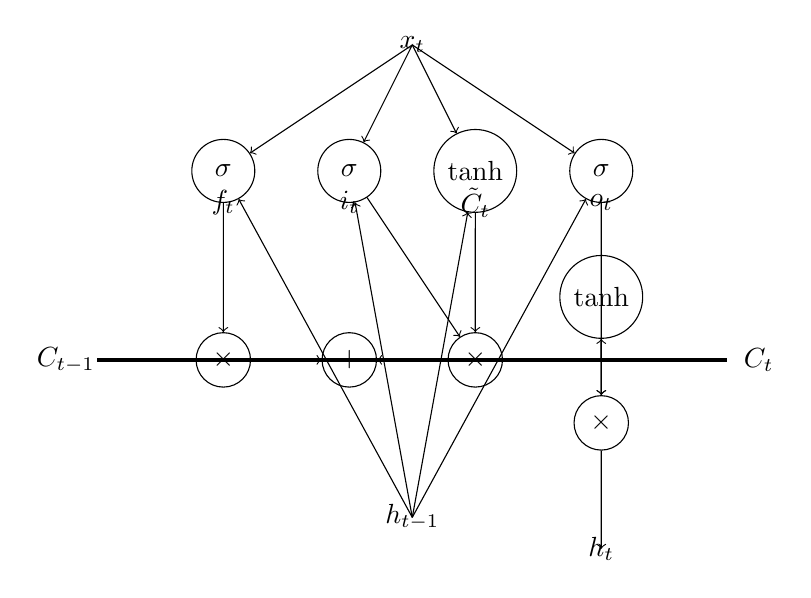
\begin{tikzpicture}[scale=0.8]
        % LSTM Cell Architecture
        \node[draw, circle, minimum size=0.8cm] (forget) at (2, 6) {$\sigma$};
        \node[draw, circle, minimum size=0.8cm] (input) at (4, 6) {$\sigma$};
        \node[draw, circle, minimum size=0.8cm] (candidate) at (6, 6) {$\tanh$};
        \node[draw, circle, minimum size=0.8cm] (output) at (8, 6) {$\sigma$};
        \node[draw, circle, minimum size=0.8cm] (final_tanh) at (8, 4) {$\tanh$};
        
        % Cell state line
        \draw[very thick] (0, 3) -- (10, 3);
        \node at (-0.5, 3) {$C_{t-1}$};
        \node at (10.5, 3) {$C_t$};
        
        % Multiplication and addition nodes
        \node[draw, circle, minimum size=0.6cm] (mult1) at (2, 3) {$\times$};
        \node[draw, circle, minimum size=0.6cm] (mult2) at (6, 3) {$\times$};
        \node[draw, circle, minimum size=0.6cm] (add) at (4, 3) {$+$};
        \node[draw, circle, minimum size=0.6cm] (mult3) at (8, 2) {$\times$};
        
        % Input and output
        \node at (5, 8) {$x_t$};
        \node at (5, 0.5) {$h_{t-1}$};
        \node at (8, 0) {$h_t$};
        
        % Connections
        \draw[->] (forget) -- (mult1);
        \draw[->] (input) -- (mult2);
        \draw[->] (candidate) -- (mult2);
        \draw[->] (mult1) -- (add);
        \draw[->] (mult2) -- (add);
        \draw[->] (output) -- (mult3);
        \draw[->] (8, 3) -- (final_tanh);
        \draw[->] (final_tanh) -- (mult3);
        \draw[->] (mult3) -- (8, 0);
        
        % Input connections
        \draw[->] (5, 8) -- (forget);
        \draw[->] (5, 8) -- (input);
        \draw[->] (5, 8) -- (candidate);
        \draw[->] (5, 8) -- (output);
        
        \draw[->] (5, 0.5) -- (forget);
        \draw[->] (5, 0.5) -- (input);
        \draw[->] (5, 0.5) -- (candidate);
        \draw[->] (5, 0.5) -- (output);
        
        % Labels
        \node at (2, 5.5) {$f_t$};
        \node at (4, 5.5) {$i_t$};
        \node at (6, 5.5) {$\tilde{C}_t$};
        \node at (8, 5.5) {$o_t$};
    \end{tikzpicture}
    \end{center}
    
    \answer{The LSTM architecture consists of three gates (forget, input, output) and two state vectors (cell state, hidden state) with specific weight matrices for each component.}
    
    \explanation{
    \textbf{Components and Information Flow:}
    \begin{itemize}
        \item \textbf{Forget Gate ($f_t$):} Controls what information to discard from cell state
        \item \textbf{Input Gate ($i_t$):} Controls what new information to store in cell state
        \item \textbf{Candidate Values ($\tilde{C}_t$):} New candidate values for cell state
        \item \textbf{Output Gate ($o_t$):} Controls what parts of cell state to output
        \item \textbf{Cell State ($C_t$):} Long-term memory, flows horizontally
        \item \textbf{Hidden State ($h_t$):} Short-term memory, filtered cell state
    \end{itemize}
    
    \textbf{Weight Matrices:}
    Each gate has input weights $W$ and recurrent weights $U$:
    $W_f, W_i, W_C, W_o$ for inputs and $U_f, U_i, U_C, U_o$ for hidden states.
    }
    
    \item Write the mathematical equations for all LSTM gates and state updates. Given input $x_t$, previous hidden state $h_{t-1}$, and previous cell state $C_{t-1}$, derive: \hfill (15 marks)
    \begin{itemize}
        \item Forget gate: $f_t = ?$
        \item Input gate: $i_t = ?$
        \item Candidate values: $\tilde{C}_t = ?$
        \item Cell state update: $C_t = ?$
        \item Output gate: $o_t = ?$
        \item Hidden state: $h_t = ?$
    \end{itemize}
    
    \answer{Complete LSTM equations with proper weight matrices and activation functions:}
    
    \explanation{
    \textbf{LSTM Mathematical Formulation:}
    
    \textbf{1. Forget Gate:} Controls what to forget from previous cell state
    $$f_t = \sigma(W_f \cdot [h_{t-1}, x_t] + b_f)$$
    
    \textbf{2. Input Gate:} Controls what new information to store
    $$i_t = \sigma(W_i \cdot [h_{t-1}, x_t] + b_i)$$
    
    \textbf{3. Candidate Values:} New candidate values to potentially store
    $$\tilde{C}_t = \tanh(W_C \cdot [h_{t-1}, x_t] + b_C)$$
    
    \textbf{4. Cell State Update:} Combines forgotten old state with new candidates
    $$C_t = f_t \odot C_{t-1} + i_t \odot \tilde{C}_t$$
    
    \textbf{5. Output Gate:} Controls what parts of cell state to output
    $$o_t = \sigma(W_o \cdot [h_{t-1}, x_t] + b_o)$$
    
    \textbf{6. Hidden State:} Filtered version of cell state
    $$h_t = o_t \odot \tanh(C_t)$$
    
    \textbf{Key Insights:}
    \begin{itemize}
        \item $\sigma$ is the sigmoid function (outputs 0-1 for gating)
        \item $\tanh$ normalizes values to [-1, 1]
        \item $\odot$ denotes element-wise multiplication
        \item $[h_{t-1}, x_t]$ represents concatenation of vectors
    \end{itemize}
    }
    
    \item Compare LSTM vs. vanilla RNN in terms of gradient flow. Explain how the cell state pathway in LSTM addresses the vanishing gradient problem through mathematical analysis of gradient propagation. \hfill (5 marks)
    
    \answer{LSTM solves vanishing gradients through the cell state pathway, which provides a highway for gradient flow with minimal transformations.}
    
    \explanation{
    \textbf{Vanilla RNN Gradient Flow:}
    For vanilla RNN: $h_t = \tanh(Wh_{t-1} + Ux_t)$
    
    Gradient through time: $\frac{\partial h_t}{\partial h_{t-k}} = \prod_{i=1}^k \frac{\partial h_{t-i+1}}{\partial h_{t-i}} = \prod_{i=1}^k W \cdot \text{diag}(\tanh'(\cdot))$
    
    Since $|\tanh'(x)| \leq 1$ and typically $<< 1$, gradients vanish exponentially.
    
    \textbf{LSTM Cell State Gradient Flow:}
    The cell state update: $C_t = f_t \odot C_{t-1} + i_t \odot \tilde{C}_t$
    
    Gradient: $\frac{\partial C_t}{\partial C_{t-1}} = f_t$ (element-wise)
    
    \textbf{Key Advantages:}
    \begin{itemize}
        \item No matrix multiplication (unlike vanilla RNN's $W$)
        \item Forget gate values can be close to 1, preserving gradients
        \item Additive updates prevent multiplicative vanishing
        \item Direct gradient pathway from $C_t$ to $C_{t-k}$ through forget gates
    \end{itemize}
    
    This creates a "gradient highway" that maintains gradient flow across long sequences.
    }
\end{enumerate}

\newpage
\paragraph{Question 3. Word Embeddings and Distributional Semantics}\hfill (22 marks)\\
Based on NLP course materials from Stanford CS224n and similar university programs.

\begin{enumerate}[(a)]
    \item Explain the distributional hypothesis that underlies word embeddings. How does the CBOW (Continuous Bag of Words) model implement this principle? \hfill (6 marks)
    
    \answer{The distributional hypothesis states that words appearing in similar contexts have similar meanings. CBOW implements this by predicting a target word from its context words.}
    
    \explanation{
    \textbf{Distributional Hypothesis:}
    "You shall know a word by the company it keeps" - words that appear in similar contexts tend to have similar meanings. This is the foundation of distributional semantics.
    
    \textbf{CBOW Implementation:}
    \begin{itemize}
        \item \textbf{Input:} Context words around target word (e.g., window size = 2)
        \item \textbf{Goal:} Predict the center word from context
        \item \textbf{Architecture:} 
        \begin{enumerate}
            \item One-hot encode context words
            \item Average their embeddings (bag of words)
            \item Use averaged embedding to predict target word
        \end{enumerate}
        \item \textbf{Learning:} Words with similar contexts get similar embeddings because they're used to predict similar target words
    \end{itemize}
    
    \textbf{Mathematical Formulation:}
    Given context words $w_{t-c}, ..., w_{t-1}, w_{t+1}, ..., w_{t+c}$:
    $$h = \frac{1}{2c} \sum_{j \neq 0, |j| \leq c} W_{embed} \cdot e_{t+j}$$
    $$P(w_t | context) = \text{softmax}(W_{out} \cdot h)$$
    }
    
    \item Design the Skip-gram model architecture for learning word embeddings. Given vocabulary size V=10,000 and embedding dimension d=300: \hfill (10 marks)
    \begin{itemize}
        \item Draw the network architecture
        \item Calculate the number of parameters
        \item Explain the softmax bottleneck and hierarchical softmax solution
        \item Derive the loss function using negative sampling
    \end{itemize}
    
    \answer{Skip-gram predicts context words from target word, with input embedding matrix $W_{in}$ (V×d) and output matrix $W_{out}$ (d×V).}
    
    \explanation{
    \textbf{Architecture:}
    \begin{center}
    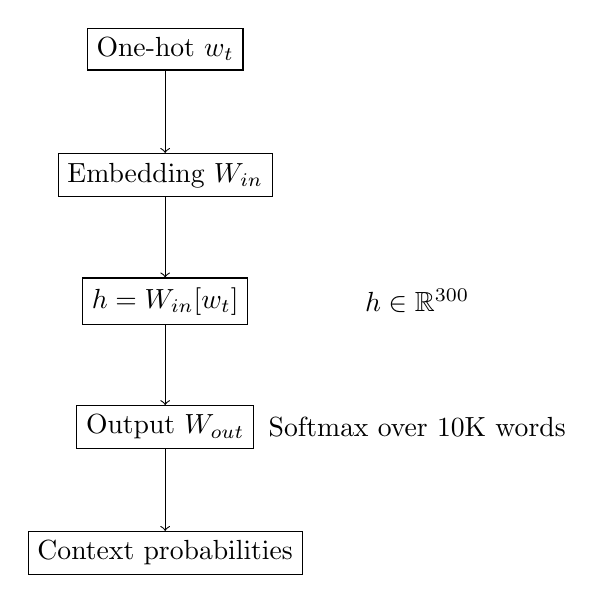
\begin{tikzpicture}[scale=0.8]
        \node[draw, rectangle] (input) at (0, 4) {One-hot $w_t$};
        \node[draw, rectangle] (embed) at (0, 2) {Embedding $W_{in}$};
        \node[draw, rectangle] (hidden) at (0, 0) {$h = W_{in}[w_t]$};
        \node[draw, rectangle] (output) at (0, -2) {Output $W_{out}$};
        \node[draw, rectangle] (context) at (0, -4) {Context probabilities};
        
        \draw[->] (input) -- (embed);
        \draw[->] (embed) -- (hidden);
        \draw[->] (hidden) -- (output);
        \draw[->] (output) -- (context);
        
        \node at (4, 0) {$h \in \mathbb{R}^{300}$};
        \node at (4, -2) {Softmax over 10K words};
    \end{tikzpicture}
    \end{center}
    
    \textbf{Parameter Count:}
    \begin{itemize}
        \item Input embedding matrix: $W_{in} = 10,000 \times 300 = 3,000,000$
        \item Output weight matrix: $W_{out} = 300 \times 10,000 = 3,000,000$
        \item Total parameters: $6,000,000$
    \end{itemize}
    
    \textbf{Softmax Bottleneck:}
    Computing softmax over 10K words is expensive: $O(V \cdot d)$ per prediction.
    
    \textbf{Hierarchical Softmax:}
    Uses binary tree structure where each word is a leaf. Path from root to leaf defines probability:
    $$P(w|context) = \prod_{i=1}^{L(w)} \sigma([[n(w,i+1) = \text{ch}(n(w,i))]] \cdot h^T \theta_{n(w,i)})$$
    Reduces complexity from $O(V)$ to $O(\log V)$.
    
    \textbf{Negative Sampling Loss:}
    For target word $w_t$ and context $w_c$:
    $$L = -\log \sigma(u_{w_c}^T v_{w_t}) - \sum_{i=1}^k \mathbb{E}_{w_i \sim P_n(w)} [\log \sigma(-u_{w_i}^T v_{w_t})]$$
    where $k$ is number of negative samples and $P_n(w)$ is noise distribution.
    }
    
    \item Analyze word embedding arithmetic: "king - man + woman ≈ queen". Explain: \hfill (6 marks)
    \begin{itemize}
        \item Why this works mathematically in embedding space
        \item What linguistic relationships are captured
        \item Limitations of linear analogies in embeddings
    \end{itemize}
    
    \answer{Word arithmetic works because embeddings capture linear relationships between semantic concepts through vector differences.}
    
    \explanation{
    \textbf{Mathematical Explanation:}
    The embedding space captures relational similarities. If we denote the relationship "male to female" as a vector $\vec{r}$, then:
    \begin{align}
        \vec{king} - \vec{man} &\approx \vec{r}_{royalty} \\
        \vec{woman} + \vec{r}_{royalty} &\approx \vec{queen}
    \end{align}
    
    The vector difference $\vec{king} - \vec{man}$ captures the "royalty" relationship, which when added to $\vec{woman}$ gives the female royal equivalent.
    
    \textbf{Linguistic Relationships Captured:}
    \begin{itemize}
        \item \textbf{Gender:} man/woman, king/queen, actor/actress
        \item \textbf{Tense:} walk/walked, go/went
        \item \textbf{Comparative:} good/better, big/bigger
        \item \textbf{Plural:} car/cars, child/children
        \item \textbf{Geography:} Paris/France, Tokyo/Japan
    \end{itemize}
    
    \textbf{Limitations:}
    \begin{itemize}
        \item \textbf{Polysemy:} Multiple word meanings not well handled
        \item \textbf{Complex Relations:} Non-linear relationships fail
        \item \textbf{Cultural Bias:} Embeddings inherit training data biases
        \item \textbf{Compositionality:} Phrase meanings don't always compose linearly
        \item \textbf{Context Independence:} Same embedding regardless of context
    \end{itemize}
    }
\end{enumerate}

\newpage
\paragraph{Question 4. Sequence-to-Sequence Models and Attention}\hfill (28 marks)\\
Based on modern NLP course materials covering encoder-decoder architectures.

\begin{enumerate}[(a)]
    \item Design an encoder-decoder RNN architecture for machine translation from English to French. Show the complete architecture including: \hfill (12 marks)
    \begin{itemize}
        \item Encoder RNN processing input sequence
        \item Context vector computation
        \item Decoder RNN generating output sequence
        \item How teacher forcing works during training
        \item Inference procedure using greedy/beam search
    \end{itemize}
    
    \answer{Encoder-decoder architecture uses two RNNs: encoder processes input sequence to create context vector, decoder generates output sequence conditioned on this context.}
    
    \explanation{
    \textbf{Complete Architecture:}
    
    \textbf{1. Encoder RNN:}
    \begin{itemize}
        \item Input: English sentence $x_1, x_2, ..., x_T$
        \item Hidden states: $h_1^{(enc)}, h_2^{(enc)}, ..., h_T^{(enc)}$
        \item Equations: $h_t^{(enc)} = f_{enc}(h_{t-1}^{(enc)}, x_t)$
    \end{itemize}
    
    \textbf{2. Context Vector:}
    \begin{itemize}
        \item Simple approach: $c = h_T^{(enc)}$ (final encoder state)
        \item Alternative: $c = \tanh(W_c h_T^{(enc)})$ (learned transformation)
    \end{itemize}
    
    \textbf{3. Decoder RNN:}
    \begin{itemize}
        \item Initial state: $h_0^{(dec)} = c$
        \item At each step: $h_t^{(dec)} = f_{dec}(h_{t-1}^{(dec)}, y_{t-1})$
        \item Output: $P(y_t) = \text{softmax}(W_o h_t^{(dec)})$
    \end{itemize}
    
    \textbf{4. Teacher Forcing (Training):}
    \begin{itemize}
        \item Use ground truth $y_{t-1}$ as input to decoder at step $t$
        \item Speeds up training and provides stable gradients
        \item Loss: $L = -\sum_{t=1}^{T'} \log P(y_t^* | y_1^*, ..., y_{t-1}^*, x)$
    \end{itemize}
    
    \textbf{5. Inference:}
    \begin{itemize}
        \item \textbf{Greedy:} Select highest probability word at each step
        \item \textbf{Beam Search:} Maintain top-k sequences, expand each
        \item Handle \textless EOS\textgreater\ token to terminate sequences
    \end{itemize}
    }
    
    \item Implement beam search decoding with beam size k=3. Given the following probability distributions over vocabulary {A, B, C, \textless EOS\textgreater} for 2 time steps: \hfill (10 marks)
    
    \begin{center}
    \begin{tabular}{|c|c|c|c|c|}
    \hline
    Context & P(A) & P(B) & P(C) & P(\textless EOS\textgreater) \\
    \hline
    Initial & 0.5 & 0.3 & 0.15 & 0.05 \\
    After A & 0.2 & 0.1 & 0.6 & 0.1 \\
    After B & 0.4 & 0.2 & 0.3 & 0.1 \\
    After C & 0.1 & 0.7 & 0.1 & 0.1 \\
    \hline
    \end{tabular}
    \end{center}
    
    Show the complete beam search tree and final ranked sequences.
    
    \answer{Beam search maintains top-3 sequences at each step, expanding each and keeping the best candidates.}
    
    \explanation{
    \textbf{Step 1: Initial Expansion}
    From \textless START\textgreater, expand to all tokens:
    \begin{itemize}
        \item A: score = 0.5
        \item B: score = 0.3  
        \item C: score = 0.15
    \end{itemize}
    Keep top 3: [A: 0.5], [B: 0.3], [C: 0.15]
    
    \textbf{Step 2: Expand Each Beam}
    
    \textbf{From A (score: 0.5):}
    \begin{itemize}
        \item AA: 0.5 × 0.2 = 0.10
        \item AB: 0.5 × 0.1 = 0.05
        \item AC: 0.5 × 0.6 = 0.30
        \item A\textless EOS\textgreater: 0.5 × 0.1 = 0.05
    \end{itemize}
    
    \textbf{From B (score: 0.3):}
    \begin{itemize}
        \item BA: 0.3 × 0.4 = 0.12
        \item BB: 0.3 × 0.2 = 0.06
        \item BC: 0.3 × 0.3 = 0.09
        \item B\textless EOS\textgreater: 0.3 × 0.1 = 0.03
    \end{itemize}
    
    \textbf{From C (score: 0.15):}
    \begin{itemize}
        \item CA: 0.15 × 0.1 = 0.015
        \item CB: 0.15 × 0.7 = 0.105
        \item CC: 0.15 × 0.1 = 0.015
        \item C\textless EOS\textgreater: 0.15 × 0.1 = 0.015
    \end{itemize}
    
    \textbf{Final Ranking (Top 3):}
    \begin{enumerate}
        \item AC: 0.30
        \item BA: 0.12
        \item CB: 0.105
    \end{enumerate}
    }
    
    \item Explain the attention mechanism as a solution to the bottleneck problem in sequence-to-sequence models. Derive the mathematical formulation for Bahdanau attention. \hfill (6 marks)
    
    \answer{Attention solves the bottleneck by allowing decoder to access all encoder states, not just the final context vector.}
    
    \explanation{
    \textbf{Bottleneck Problem:}
    Standard seq2seq compresses entire input sequence into fixed-size context vector $c = h_T^{(enc)}$. This creates information loss for long sequences and makes it difficult to align input-output positions.
    
    \textbf{Attention Solution:}
    Instead of single context vector, compute different context vector $c_t$ at each decoder step based on all encoder states.
    
    \textbf{Bahdanau Attention Formulation:}
    
    \textbf{1. Attention Scores:}
    $$e_{t,j} = a(h_{t-1}^{(dec)}, h_j^{(enc)})$$
    where $a$ is alignment model: $a(h_{t-1}^{(dec)}, h_j^{(enc)}) = v_a^T \tanh(W_a h_{t-1}^{(dec)} + U_a h_j^{(enc)})$
    
    \textbf{2. Attention Weights:}
    $$\alpha_{t,j} = \frac{\exp(e_{t,j})}{\sum_{k=1}^T \exp(e_{t,k})}$$
    
    \textbf{3. Context Vector:}
    $$c_t = \sum_{j=1}^T \alpha_{t,j} h_j^{(enc)}$$
    
    \textbf{4. Decoder Update:}
    $$h_t^{(dec)} = f_{dec}(h_{t-1}^{(dec)}, y_{t-1}, c_t)$$
    
    \textbf{Key Benefits:}
    \begin{itemize}
        \item No information bottleneck
        \item Automatic alignment learning
        \item Interpretable attention weights
        \item Better handling of long sequences
    \end{itemize}
    }
\end{enumerate}

\newpage
\paragraph{Question 5. Gradient Problems and Solutions}\hfill (20 marks)\\
Based on theoretical analysis from university deep learning courses.

\begin{enumerate}[(a)]
    \item Analyze the vanishing gradient problem in RNNs. For an RNN with hidden state transition $h_t = \tanh(W h_{t-1} + U x_t)$, show mathematically why gradients vanish for long sequences. \hfill (8 marks)
    
    Include analysis of:
    \begin{itemize}
        \item Gradient computation through multiple time steps
        \item Effect of tanh derivative bounds
        \item Impact of weight matrix eigenvalues
    \end{itemize}
    
    \answer{Gradients vanish due to repeated multiplication of small derivatives and weight matrices with eigenvalues less than 1.}
    
    \explanation{
    \textbf{Gradient Computation Through Time:}
    
    For loss at time $t$, gradient w.r.t. hidden state at time $t-k$:
    $$\frac{\partial L_t}{\partial h_{t-k}} = \frac{\partial L_t}{\partial h_t} \prod_{i=1}^k \frac{\partial h_{t-i+1}}{\partial h_{t-i}}$$
    
    \textbf{Individual Gradient Term:}
    $$\frac{\partial h_{t-i+1}}{\partial h_{t-i}} = \frac{\partial \tanh(W h_{t-i} + U x_{t-i+1})}{\partial h_{t-i}} = W \cdot \text{diag}(\tanh'(W h_{t-i} + U x_{t-i+1}))$$
    
    \textbf{Effect of Tanh Derivative:}
    Since $\tanh'(x) = 1 - \tanh^2(x)$ and $|\tanh(x)| \leq 1$:
    \begin{itemize}
        \item $\tanh'(x) \in [0, 1]$
        \item For saturated regions: $\tanh'(x) \approx 0$
        \item Maximum at $x = 0$: $\tanh'(0) = 1$
    \end{itemize}
    
    \textbf{Complete Gradient:}
    $$\frac{\partial L_t}{\partial h_{t-k}} = \frac{\partial L_t}{\partial h_t} \prod_{i=1}^k W \cdot \text{diag}(\tanh'(\cdot))$$
    
    \textbf{Why Gradients Vanish:}
    \begin{itemize}
        \item \textbf{Derivative bounds:} Each $\tanh'(\cdot) \leq 1$, typically much smaller
        \item \textbf{Matrix multiplication:} If largest eigenvalue $\lambda_{max}(W) < 1$, then $\|W^k\|$ decays exponentially
        \item \textbf{Combined effect:} Product of $k$ terms, each $\leq 1$, causes exponential decay
    \end{itemize}
    
    \textbf{Mathematical Bound:}
    $$\left\|\frac{\partial L_t}{\partial h_{t-k}}\right\| \leq \left\|\frac{\partial L_t}{\partial h_t}\right\| \cdot \gamma^k$$
    where $\gamma = \lambda_{max}(W) \cdot \max_i(\tanh'(\cdot))$ and typically $\gamma < 1$.
    }
    
    \item Compare three solutions to gradient problems in RNNs: \hfill (12 marks)
    \begin{itemize}
        \item Gradient clipping (explain algorithm and threshold selection)
        \item LSTM gating mechanisms (focus on gradient flow)
        \item Skip connections in deep RNNs
    \end{itemize}
    
    Provide mathematical justification for each approach.
    
    \answer{Three complementary solutions: gradient clipping prevents explosion, LSTM gates enable selective flow, skip connections provide direct paths.}
    
    \explanation{
    \textbf{1. Gradient Clipping:}
    
    \textbf{Algorithm:}
    \begin{algorithmic}
    \STATE Compute gradient $g = \nabla_\theta L$
    \STATE Compute gradient norm $\|g\|$
    \IF{$\|g\| > \text{threshold}$}
        \STATE $g \leftarrow \frac{\text{threshold}}{\|g\|} \cdot g$
    \ENDIF
    \STATE Update parameters: $\theta \leftarrow \theta - \alpha g$
    \end{algorithmic}
    
    \textbf{Threshold Selection:}
    \begin{itemize}
        \item Monitor gradient norms during training
        \item Choose threshold as 95th percentile of observed norms
        \item Typical values: 1.0-5.0 for RNNs
    \end{itemize}
    
    \textbf{Mathematical Justification:}
    Prevents parameter updates that are too large: $\|\Delta \theta\| = \alpha \|g\| \leq \alpha \cdot \text{threshold}$
    
    \textbf{2. LSTM Gating Mechanisms:}
    
    \textbf{Gradient Flow Analysis:}
    Cell state gradient: $\frac{\partial C_t}{\partial C_{t-1}} = f_t$
    
    Unlike vanilla RNN, no matrix multiplication or bounded activation in the direct path.
    
    \textbf{Key Properties:}
    \begin{itemize}
        \item \textbf{Forget gate values:} Can be close to 1, preserving gradients
        \item \textbf{Additive updates:} $C_t = f_t \odot C_{t-1} + i_t \odot \tilde{C}_t$
        \item \textbf{Selective information flow:} Gates learn when to preserve/update
    \end{itemize}
    
    \textbf{3. Skip Connections in Deep RNNs:}
    
    \textbf{Architecture:}
    $$h_t^{(l)} = f(h_t^{(l-1)}, h_{t-1}^{(l)}) + h_t^{(l-1)}$$
    
    \textbf{Gradient Flow:}
    $$\frac{\partial h_t^{(l)}}{\partial h_t^{(l-1)}} = \frac{\partial f}{\partial h_t^{(l-1)}} + I$$
    
    The identity term $I$ provides direct gradient flow, preventing vanishing even if $\frac{\partial f}{\partial h_t^{(l-1)}}$ is small.
    
    \textbf{Benefits:}
    \begin{itemize}
        \item Direct gradient pathways across layers
        \item Improved training stability
        \item Better information flow in deep architectures
    \end{itemize}
    }
\end{enumerate}

\newpage
\paragraph{Question 6. Language Modeling Evaluation and Perplexity}\hfill (18 marks)\\
Based on NLP evaluation metrics taught in university courses.

\begin{enumerate}[(a)]
    \item Define perplexity as a measure of language model quality. Given a test sequence $w_1, w_2, \ldots, w_N$, derive the relationship between perplexity and cross-entropy loss. \hfill (8 marks)
    
    \answer{Perplexity measures how well a language model predicts a text sequence, mathematically defined as the exponential of average cross-entropy.}
    
    \explanation{
    \textbf{Perplexity Definition:}
    Perplexity measures the uncertainty or "surprise" of a language model when predicting text. Lower perplexity indicates better model performance.
    
    \textbf{Mathematical Derivation:}
    
    \textbf{1. Probability of Sequence:}
    $$P(w_1, w_2, \ldots, w_N) = \prod_{i=1}^N P(w_i | w_1, \ldots, w_{i-1})$$
    
    \textbf{2. Log-likelihood:}
    $$\log P(w_1, \ldots, w_N) = \sum_{i=1}^N \log P(w_i | w_1, \ldots, w_{i-1})$$
    
    \textbf{3. Cross-entropy Loss:}
    $$H = -\frac{1}{N} \sum_{i=1}^N \log P(w_i | w_1, \ldots, w_{i-1})$$
    
    \textbf{4. Perplexity:}
    $$\text{PPL} = 2^H = 2^{-\frac{1}{N} \sum_{i=1}^N \log_2 P(w_i | w_1, \ldots, w_{i-1})}$$
    
    Or equivalently: $\text{PPL} = \left(\prod_{i=1}^N P(w_i | w_1, \ldots, w_{i-1})\right)^{-1/N}$
    
    \textbf{Relationship:}
    $$\text{Perplexity} = 2^{\text{Cross-entropy}}$$
    
    \textbf{Intuition:} Perplexity represents the effective vocabulary size - a perplexity of 100 means the model is as confused as if it had to choose uniformly among 100 words at each step.
    }
    
    \item A character-level RNN language model with vocabulary size 50 achieves the following results: \hfill (10 marks)
    \begin{itemize}
        \item Training perplexity: 1.8
        \item Validation perplexity: 2.3
        \item Test perplexity: 2.5
    \end{itemize}
    
    \begin{itemize}
        \item Calculate the average bits per character for each dataset
        \item Analyze what these results indicate about model performance
        \item Compare with a baseline uniform model (calculate its perplexity)
        \item Suggest improvements to reduce the validation-test gap
    \end{itemize}
    
    \answer{Bits per character calculated using log₂ of perplexity; results show good training but some overfitting compared to uniform baseline.}
    
    \explanation{
    \textbf{1. Bits Per Character Calculation:}
    Since $\text{PPL} = 2^{\text{Cross-entropy}}$, we have $\text{Cross-entropy} = \log_2(\text{PPL})$:
    
    \begin{itemize}
        \item Training: $\log_2(1.8) = 0.85$ bits/char
        \item Validation: $\log_2(2.3) = 1.20$ bits/char  
        \item Test: $\log_2(2.5) = 1.32$ bits/char
    \end{itemize}
    
    \textbf{2. Performance Analysis:}
    \begin{itemize}
        \item \textbf{Good Training Performance:} PPL of 1.8 is quite good for character-level modeling
        \item \textbf{Moderate Overfitting:} Validation PPL (2.3) > Training PPL (1.8), indicating some overfitting
        \item \textbf{Generalization Gap:} Test PPL (2.5) slightly higher than validation, suggesting model generalizes reasonably well
        \item \textbf{Overall Assessment:} Model has learned meaningful patterns but could benefit from regularization
    \end{itemize}
    
    \textbf{3. Uniform Baseline:}
    For uniform distribution over 50 characters:
    $$P_{\text{uniform}}(c) = \frac{1}{50} = 0.02$$
    $$\text{PPL}_{\text{uniform}} = 50$$
    $$\text{Bits per char}_{\text{uniform}} = \log_2(50) = 5.64 \text{ bits/char}$$
    
    Our model (1.32 bits/char) significantly outperforms uniform baseline (5.64 bits/char).
    
    \textbf{4. Suggested Improvements:}
    \begin{itemize}
        \item \textbf{Regularization:} Add dropout, weight decay, or early stopping
        \item \textbf{Data Augmentation:} Increase training data diversity
        \item \textbf{Architecture:} Try LSTM/GRU or deeper networks
        \item \textbf{Hyperparameter Tuning:} Optimize learning rate, hidden size
        \item \textbf{Ensemble Methods:} Combine multiple models
        \item \textbf{Better Preprocessing:} Improved tokenization or normalization
    \end{itemize}
    }
\end{enumerate}

\newpage
\paragraph{Question 7. Modern RNN Variants and Applications}\hfill (27 marks)\\
Based on advanced topics from recent university deep learning curricula.

\begin{enumerate}[(a)]
    \item Compare GRU (Gated Recurrent Unit) with LSTM architecture. Draw both architectures and explain: \hfill (12 marks)
    \begin{itemize}
        \item Key architectural differences
        \item Parameter count comparison
        \item Computational efficiency analysis
        \item When to choose GRU vs LSTM
    \end{itemize}
    
    \answer{GRU simplifies LSTM by combining forget and input gates into update gate and merging cell/hidden states.}
    
    \explanation{
    \textbf{GRU Architecture:}
    \begin{center}
    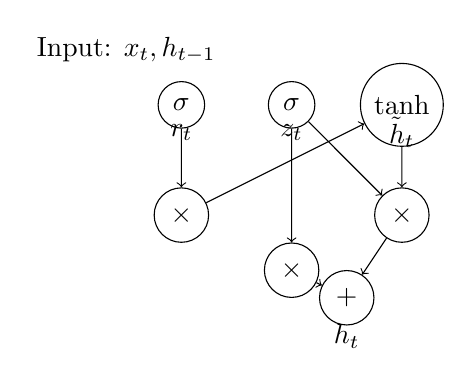
\begin{tikzpicture}[scale=0.7]
        % GRU Components
        \node[draw, circle] (reset) at (1, 4) {$\sigma$};
        \node[draw, circle] (update) at (3, 4) {$\sigma$};
        \node[draw, circle] (candidate) at (5, 4) {$\tanh$};
        \node[draw, circle] (mult1) at (1, 2) {$\times$};
        \node[draw, circle] (mult2) at (5, 2) {$\times$};
        \node[draw, circle] (mult3) at (3, 1) {$\times$};
        \node[draw, circle] (add) at (4, 0.5) {$+$};
        
        \draw[->] (reset) -- (mult1);
        \draw[->] (mult1) -- (candidate);
        \draw[->] (candidate) -- (mult2);
        \draw[->] (update) -- (mult2);
        \draw[->] (update) -- (mult3);
        \draw[->] (mult2) -- (add);
        \draw[->] (mult3) -- (add);
        
        \node at (1, 3.5) {$r_t$};
        \node at (3, 3.5) {$z_t$};
        \node at (5, 3.5) {$\tilde{h}_t$};
        \node at (0, 5) {Input: $x_t, h_{t-1}$};
        \node at (4, -0.2) {$h_t$};
    \end{tikzpicture}
    \end{center}
    
    \textbf{GRU Equations:}
    \begin{align}
        r_t &= \sigma(W_r \cdot [h_{t-1}, x_t]) \quad \text{(reset gate)} \\
        z_t &= \sigma(W_z \cdot [h_{t-1}, x_t]) \quad \text{(update gate)} \\
        \tilde{h}_t &= \tanh(W_h \cdot [r_t \odot h_{t-1}, x_t]) \quad \text{(candidate)} \\
        h_t &= (1-z_t) \odot h_{t-1} + z_t \odot \tilde{h}_t \quad \text{(final state)}
    \end{align}
    
    \textbf{Key Architectural Differences:}
    \begin{itemize}
        \item \textbf{States:} LSTM has separate cell/hidden states; GRU combines them
        \item \textbf{Gates:} LSTM has 3 gates (forget, input, output); GRU has 2 (reset, update)
        \item \textbf{Memory:} LSTM explicit memory cell; GRU implicit in hidden state
        \item \textbf{Control:} GRU update gate controls both forget and input simultaneously
    \end{itemize}
    
    \textbf{Parameter Count Comparison:}
    For hidden size $h$ and input size $d$:
    \begin{itemize}
        \item \textbf{LSTM:} $4 \times (h \times (h + d) + h) = 4h(h + d + 1)$ parameters
        \item \textbf{GRU:} $3 \times (h \times (h + d) + h) = 3h(h + d + 1)$ parameters
        \item \textbf{Reduction:} GRU has 25\% fewer parameters
    \end{itemize}
    
    \textbf{Computational Efficiency:}
    \begin{itemize}
        \item \textbf{GRU:} Fewer matrix multiplications, faster training/inference
        \item \textbf{LSTM:} More complex gating, higher memory requirements
        \item \textbf{Practical difference:} 10-15\% speedup with GRU
    \end{itemize}
    
    \textbf{When to Choose:}
    \begin{itemize}
        \item \textbf{Choose GRU:} Limited data, computational constraints, simpler sequences
        \item \textbf{Choose LSTM:} Complex long-term dependencies, sufficient data, need explicit memory control
    \end{itemize}
    }
    
    \item Design a bidirectional RNN for named entity recognition. Explain: \hfill (8 marks)
    \begin{itemize}
        \item Forward and backward pass computations
        \item How to combine directional information
        \item Advantages for sequence labeling tasks
        \item Training considerations
    \end{itemize}
    
    \answer{Bidirectional RNN processes sequence in both directions, combining forward and backward hidden states for each position.}
    
    \explanation{
    \textbf{Architecture for NER:}
    
    \textbf{1. Forward Pass:}
    $$\overrightarrow{h}_t = f(\overrightarrow{h}_{t-1}, x_t), \quad t = 1, 2, \ldots, T$$
    
    \textbf{2. Backward Pass:}
    $$\overleftarrow{h}_t = f(\overleftarrow{h}_{t+1}, x_t), \quad t = T, T-1, \ldots, 1$$
    
    \textbf{3. Combine Directional Information:}
    Several approaches:
    \begin{itemize}
        \item \textbf{Concatenation:} $h_t = [\overrightarrow{h}_t; \overleftarrow{h}_t]$
        \item \textbf{Sum:} $h_t = \overrightarrow{h}_t + \overleftarrow{h}_t$
        \item \textbf{Element-wise Product:} $h_t = \overrightarrow{h}_t \odot \overleftarrow{h}_t$
        \item \textbf{Learned Combination:} $h_t = W_f \overrightarrow{h}_t + W_b \overleftarrow{h}_t$
    \end{itemize}
    
    \textbf{4. NER Prediction:}
    $$P(\text{label}_t) = \text{softmax}(W_o h_t + b_o)$$
    
    \textbf{Advantages for Sequence Labeling:}
    \begin{itemize}
        \item \textbf{Full Context:} Access to both past and future context
        \item \textbf{Better Boundaries:} Can identify entity boundaries more accurately
        \item \textbf{Disambiguation:} Context from both directions helps resolve ambiguity
        \item \textbf{Example:} "Bank of America" - forward sees "Bank", backward sees "America"
    \end{itemize}
    
    \textbf{Training Considerations:}
    \begin{itemize}
        \item \textbf{Memory:} Double the memory requirement for hidden states
        \item \textbf{Parallelization:} Forward and backward passes can be computed in parallel
        \item \textbf{Gradient Flow:} Gradients flow through both directions
        \item \textbf{Loss Function:} Standard cross-entropy with BIO/BILOU tagging scheme
    \end{itemize}
    }
    
    \item Analyze the computational complexity of different RNN variants: \hfill (7 marks)
    
    \begin{center}
    \begin{tabular}{|l|c|c|c|}
    \hline
    Model & Time Complexity & Space Complexity & Parameters \\
    \hline
    Vanilla RNN & ? & ? & ? \\
    LSTM & ? & ? & ? \\
    GRU & ? & ? & ? \\
    Bidirectional LSTM & ? & ? & ? \\
    \hline
    \end{tabular}
    \end{center}
    
    For sequence length T, hidden size H, and input size D.
    
    \answer{Complexity analysis shows linear scaling with sequence length, with LSTM/GRU having higher constants due to gating operations.}
    
    \explanation{
    \textbf{Complexity Analysis:}
    
    \begin{center}
    \begin{tabular}{|l|c|c|c|}
    \hline
    Model & Time Complexity & Space Complexity & Parameters \\
    \hline
    Vanilla RNN & $O(T \cdot H^2 + T \cdot H \cdot D)$ & $O(T \cdot H)$ & $O(H^2 + H \cdot D)$ \\
    LSTM & $O(T \cdot 4H^2 + T \cdot 4H \cdot D)$ & $O(T \cdot 2H)$ & $O(4H^2 + 4H \cdot D)$ \\
    GRU & $O(T \cdot 3H^2 + T \cdot 3H \cdot D)$ & $O(T \cdot H)$ & $O(3H^2 + 3H \cdot D)$ \\
    Bidirectional LSTM & $O(T \cdot 8H^2 + T \cdot 8H \cdot D)$ & $O(T \cdot 4H)$ & $O(8H^2 + 8H \cdot D)$ \\
    \hline
    \end{tabular}
    \end{center}
    
    \textbf{Detailed Breakdown:}
    
    \textbf{Time Complexity Components:}
    \begin{itemize}
        \item \textbf{Hidden-to-hidden:} $H \times H$ matrix multiplication at each step
        \item \textbf{Input-to-hidden:} $D \times H$ matrix multiplication at each step
        \item \textbf{Multiple gates:} Factor of 4 for LSTM, 3 for GRU
        \item \textbf{Sequence length:} Linear factor of $T$
    \end{itemize}
    
    \textbf{Space Complexity:}
    \begin{itemize}
        \item \textbf{Hidden states:} Store $H$ values per time step
        \item \textbf{LSTM cell states:} Additional $H$ values per time step
        \item \textbf{Bidirectional:} Double the space for both directions
    \end{itemize}
    
    \textbf{Parameter Scaling:}
    \begin{itemize}
        \item Parameters scale with $H^2$ (dominant term for large $H$)
        \item Input contribution scales with $H \cdot D$
        \item Gate multipliers: 4 for LSTM, 3 for GRU
    \end{itemize}
    
    \textbf{Practical Implications:}
    \begin{itemize}
        \item LSTM/GRU are 3-4x more expensive than vanilla RNN
        \item Bidirectional models double the computational cost
        \item Memory requirements can be significant for long sequences
    \end{itemize}
    }
\end{enumerate}

\vfill
\begin{center}{\bf END OF PAPER}\end{center}
\end{document}